\subsection{Optymalizacja obliczeń matematycznych}
\thispagestyle{empty}
\par\indent

Renderując dużą ilość niewielkich obiektów należy pamiętać o optymalizacji obliczeń jeszcze przed samym renderingiem sceny. Obliczenia na liczbach zmiennoprzecinkowych oraz macierzach zużywają znaczącą ilość czasu procesora. 

\subsubsection{Program początkowy}
\thispagestyle{empty}
\par\indent

Już na tym etapie można zyskać znaczną poprawę czasu renderowania.  W tym przypadku wyświetlanych będzie 20000 sześcianów, które obracane są względem osi pionwej. Dane wierzchołków (położenie oraz kolor) dla wszystkich sześcianów są takie same. Informacje o przesunięciu oraz obrocie sześciany przekazywane są do wbudowanego w OpenGL procesu renderującego.

\lstinputlisting[language=c++,caption=Algorytm dynamicznie renderujący sześciany]{sources/unoptimized_rendering_loop.cpp}
\lstinputlisting[language=c++,caption=Algorytm obliczania docelowego położenia każdego wierzchołka]{sources/basic_vertex_shader.shader}
\lstinputlisting[language=c++,caption=Algorytm obliczenia koloru wierzchołka]{sources/basic_fragment_shader.shader}

Jak widzimy wszystkie obliczenia powtarzane są dla każdego sześcianu. Taka struktura programu owocuje długim czasem renderowania każdej klatki który trwa średnio 0.6 sekundy. Daje to około 16 klatek w cięgu 10 sekund.

\begin{figure}[h]
	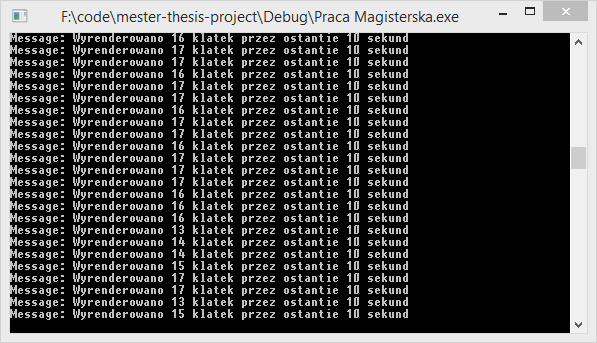
\includegraphics[width=\textwidth]{images/optimized0_console}
	\caption{Inforamcje diagnostyczne}
\end{figure}


\subsubsection{Usunięcie zbędnych obliczeń na macierzach}
\thispagestyle{empty}
\par\indent

Warto tutaj zauważyć, że macierz projekcji oraz widoku jest taka sama dla każdego wierzchołka. Może zmienić się ona co najwyżej raz dla każdej klatki. Dlatego warto przemieść obliczanie ich ilorazu na początek pętli renderującej klatkę. Nie wprowadzi to potrzeby zmian w obliczeniach per wierzchołek.

\lstinputlisting[language=c++,caption=Pętla renderująca]{sources/optimized_matrix_operations.cpp}

\begin{figure}[h]
	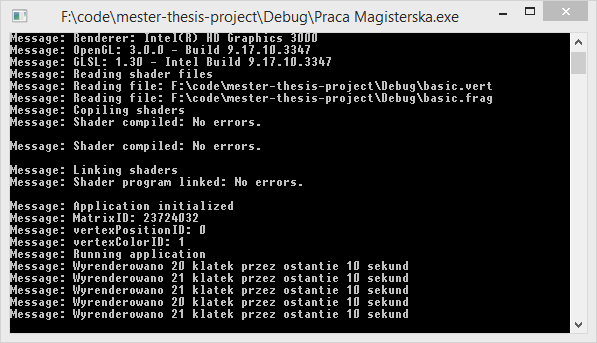
\includegraphics[width=\textwidth]{images/optimized1_console}
	\caption{Inforamcje diagnostyczne}
\end{figure}


\subsubsection{Przeniesienie obliczeń do Shadera}
\thispagestyle{empty}
\par\indent

Kolejnym krokiem w optymalizacji obliczeń jest przeniesienie operacji na macierzach do jednostek obliczeniowych znajdujących się na  karcie graficznej. Jak zostało wspomniane w poprzednich rozdziałach GPU został zaprojektowany do wykonywania obliczeń zmiennoprzecinkowych. Dodatkowo odciąży to jednostkę CPU i skróci czas wykonywania kolejnych obrotów pętli.

Aby tego dokonać należy zmodyfikować vertex shader aby akceptował dodatkowy parametr oraz wykonywał niezbędne obliczenia.

\lstinputlisting[language=c,caption=Vertex Shader]{sources/vertex_shader_with_additional_matrix.shader}

Następnie należy odpowiednio zmodyfikować pętle renderrujące sześciany.

\lstinputlisting[language=c,caption=Pętla renderująca]{sources/rendering_loop_wo_matrix_operations.cpp}

Wzrost wydajności znowu jest znaczący. Czas wymagany do wykonania wszystkich obliczeń per klatka zmniejszył się do 0.34 sekundy. Pozwala to na wyświetlenie średnio 28 klatek w czasie 10 sekund.

\begin{figure}[h]
	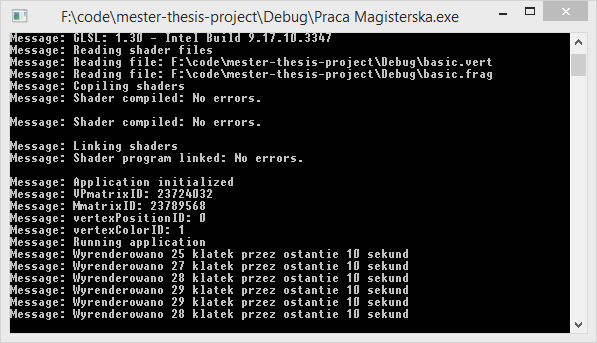
\includegraphics[width=\textwidth]{images/optimized2_console}
	\caption{Inforamcje diagnostyczne}
\end{figure}


\subsubsection{Zmniejszenie liczby operacji macierzowych}
\thispagestyle{empty}
\par\indent

W obecny stanie uzyskaliśmy znaczny wzrost wydajności. Jednak wciąż pewne obliczenia są zbędnie powtarzane dla każdego sześcianu. Warto tuatj zauwazyć, że wszystkie obiekty obracają się w tym samym kierunku, z tą samą prędkością oraz w okół tej samej osi. Daje nam to kolejną możliwość zmniejszenia czasu potrzebnego do wykonania wszysktkich niezbędnych obliczeń.

Dodatkowo mając doświadczenia z poprzednich kroków wiemy, że dobrym posunięciem będzie przeniesienie aplikowania macierzy obrotu do vertex shadera.

\lstinputlisting[language=c,caption=Vertex Shader]{sources/vertex_shader_with_rotation_matrix.shader}
\lstinputlisting[language=c,caption=Pętla renderująca]{sources/rendering_loop_wo_rotation_matrix.cpp}

\begin{figure}[h]
	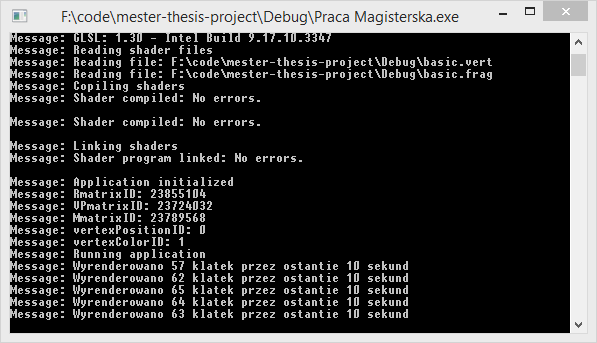
\includegraphics[width=\textwidth]{images/optimized3_console}
	\caption{Inforamcje diagnostyczne}
\end{figure}

Jak widać w tym przypadku wzrost wydajności jest znaczący. Od W stosunku do poprzedniej wersji udało się skrócić czas renderowania jednej klatki o połowę. Ten przykład pokazuje jak bardzo krytyczny jest dobór miejsca gdzie przeprowadzane są obliczenia zmiennoprzecinkowe.

\subsubsection{Minimalizowanie ilości odwołań do shadera}
\thispagestyle{empty}
\par\indent

O ile przeniesienie obliczeń do procesora GPU może okazać się zbawienne w czasie wykonywania obliczeń. To już ilość odwołań do steronika czy to do przesyłania danych lub pobierania informacji o aktualnym stanie OpenGL jest kosztowne.

Warto też zauważyć, że dla każdego z renderowanych obiektów dane przesyłane do shaderów nie zmieniają się. Wywoływanie metod z OpenGL API za każdym razem jest zbędne i prowadzi do znacznego spadku wydajności.

\lstinputlisting[language=c,caption=Pętla renderująca]{sources/rendering_loop_wo_api_calls.cpp}

Sama zmiana jest dość subtelna i nie rzutuje na ilość obliczeń wykonywanych przez CPU. Jednak powszechnie wiadomo, że wywołanie każdej metody czy to z własnego programu czy odwołanie się do zewnętrznych bibliotek skutkuje pwnym narzutem wydajnościowym.

\begin{figure}[h]
	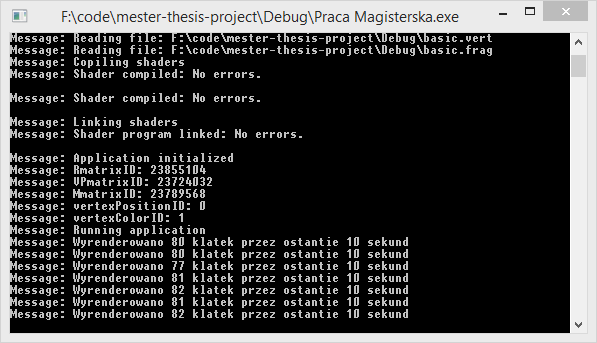
\includegraphics[width=\textwidth]{images/optimized4_console}
	\caption{Inforamcje diagnostyczne}
\end{figure}

Jak w tym przypadku widać przez tak drobną zmianę zyskaliśmy niemal 30\% wzrostu wydajności względem poprzednich pomiarów. Jest to znacząca ilość względem dokonanych zmian. Pomimo swojej wydajności należy ograniczyć ilość odwołań do jednostki GPU.


\subsubsection{Wnioski}
\thispagestyle{empty}
\par\indent

Dzięki powyższym zabiegom otrzymaliśmy czerokrotny wzrost wydajności. Czas renderowania jednej klatki został drastycznie zmniejszony. Warto tuatj zauwazyć, iż dobór miejsca wykonywania operacji matematycznych jest niezwykle ważny. Przede wszystkiem nie powinny znajdować się one w pętlach jeżeli nie jest to koneiczne. Gdy istneije taka możliwość powinny być one wykonywane przez jednostkę specjalnie zaprojektowaną do tego celu, dla liczb zmiennoprzecinkowych GPU, a dla stałoprzecinkowych CPU.

Proces optymalizacji tego fragmentu kodu można uznać jako niepełny ponieważ znajjdują się w nim operacje macierzowe wykonywane przez CPU. Jendka nie można ich zlikwidować ponieważ renderowane obiekty tworzone są dynamicznie. Proces przenoszenia operacji tworzenia  macierzy modelu do jednostki GPU nie dałby oczekiwanych rezultatów. Argumentem za tym ztojącym jest fakt iż dla każdego wierzchołka dana macierz byłaby tworzona niealeznie. Co za tym idzie wzrósłby narzut pamięciowy oraz obliczeniowy.
